%%%%%%%%%%%%%%%%%%%%%%%%%%%%%%%%%%%%%%%%%%
%%%%%%%%%%%%%                 %%%%%%%%%%%%
%%%%%%%%%%%%%    EXERCISE 1   %%%%%%%%%%%%
%%%%%%%%%%%%%                 %%%%%%%%%%%%
%%%%%%%%%%%%%%%%%%%%%%%%%%%%%%%%%%%%%%%%%%
\begin{exercise}[]{Simulate the following topology in Mininet. Set the link bandwidth for (s1,s2) and (s1,s3) as 10Mbps. Use iperf3 to test the TCP throughput between h1 to h2, h3, h4.(30 points)
    }
  \begin{solution}
  \par{~}
  \end{solution}

The TCP throughput between h1 to h2, h3, h4 is 18.3, 17.1 and 25.0 Gbits/sec respectively, shown in Figure \ref{fig:ex1}.

\begin{figure}[hb]
  \begin{center}
  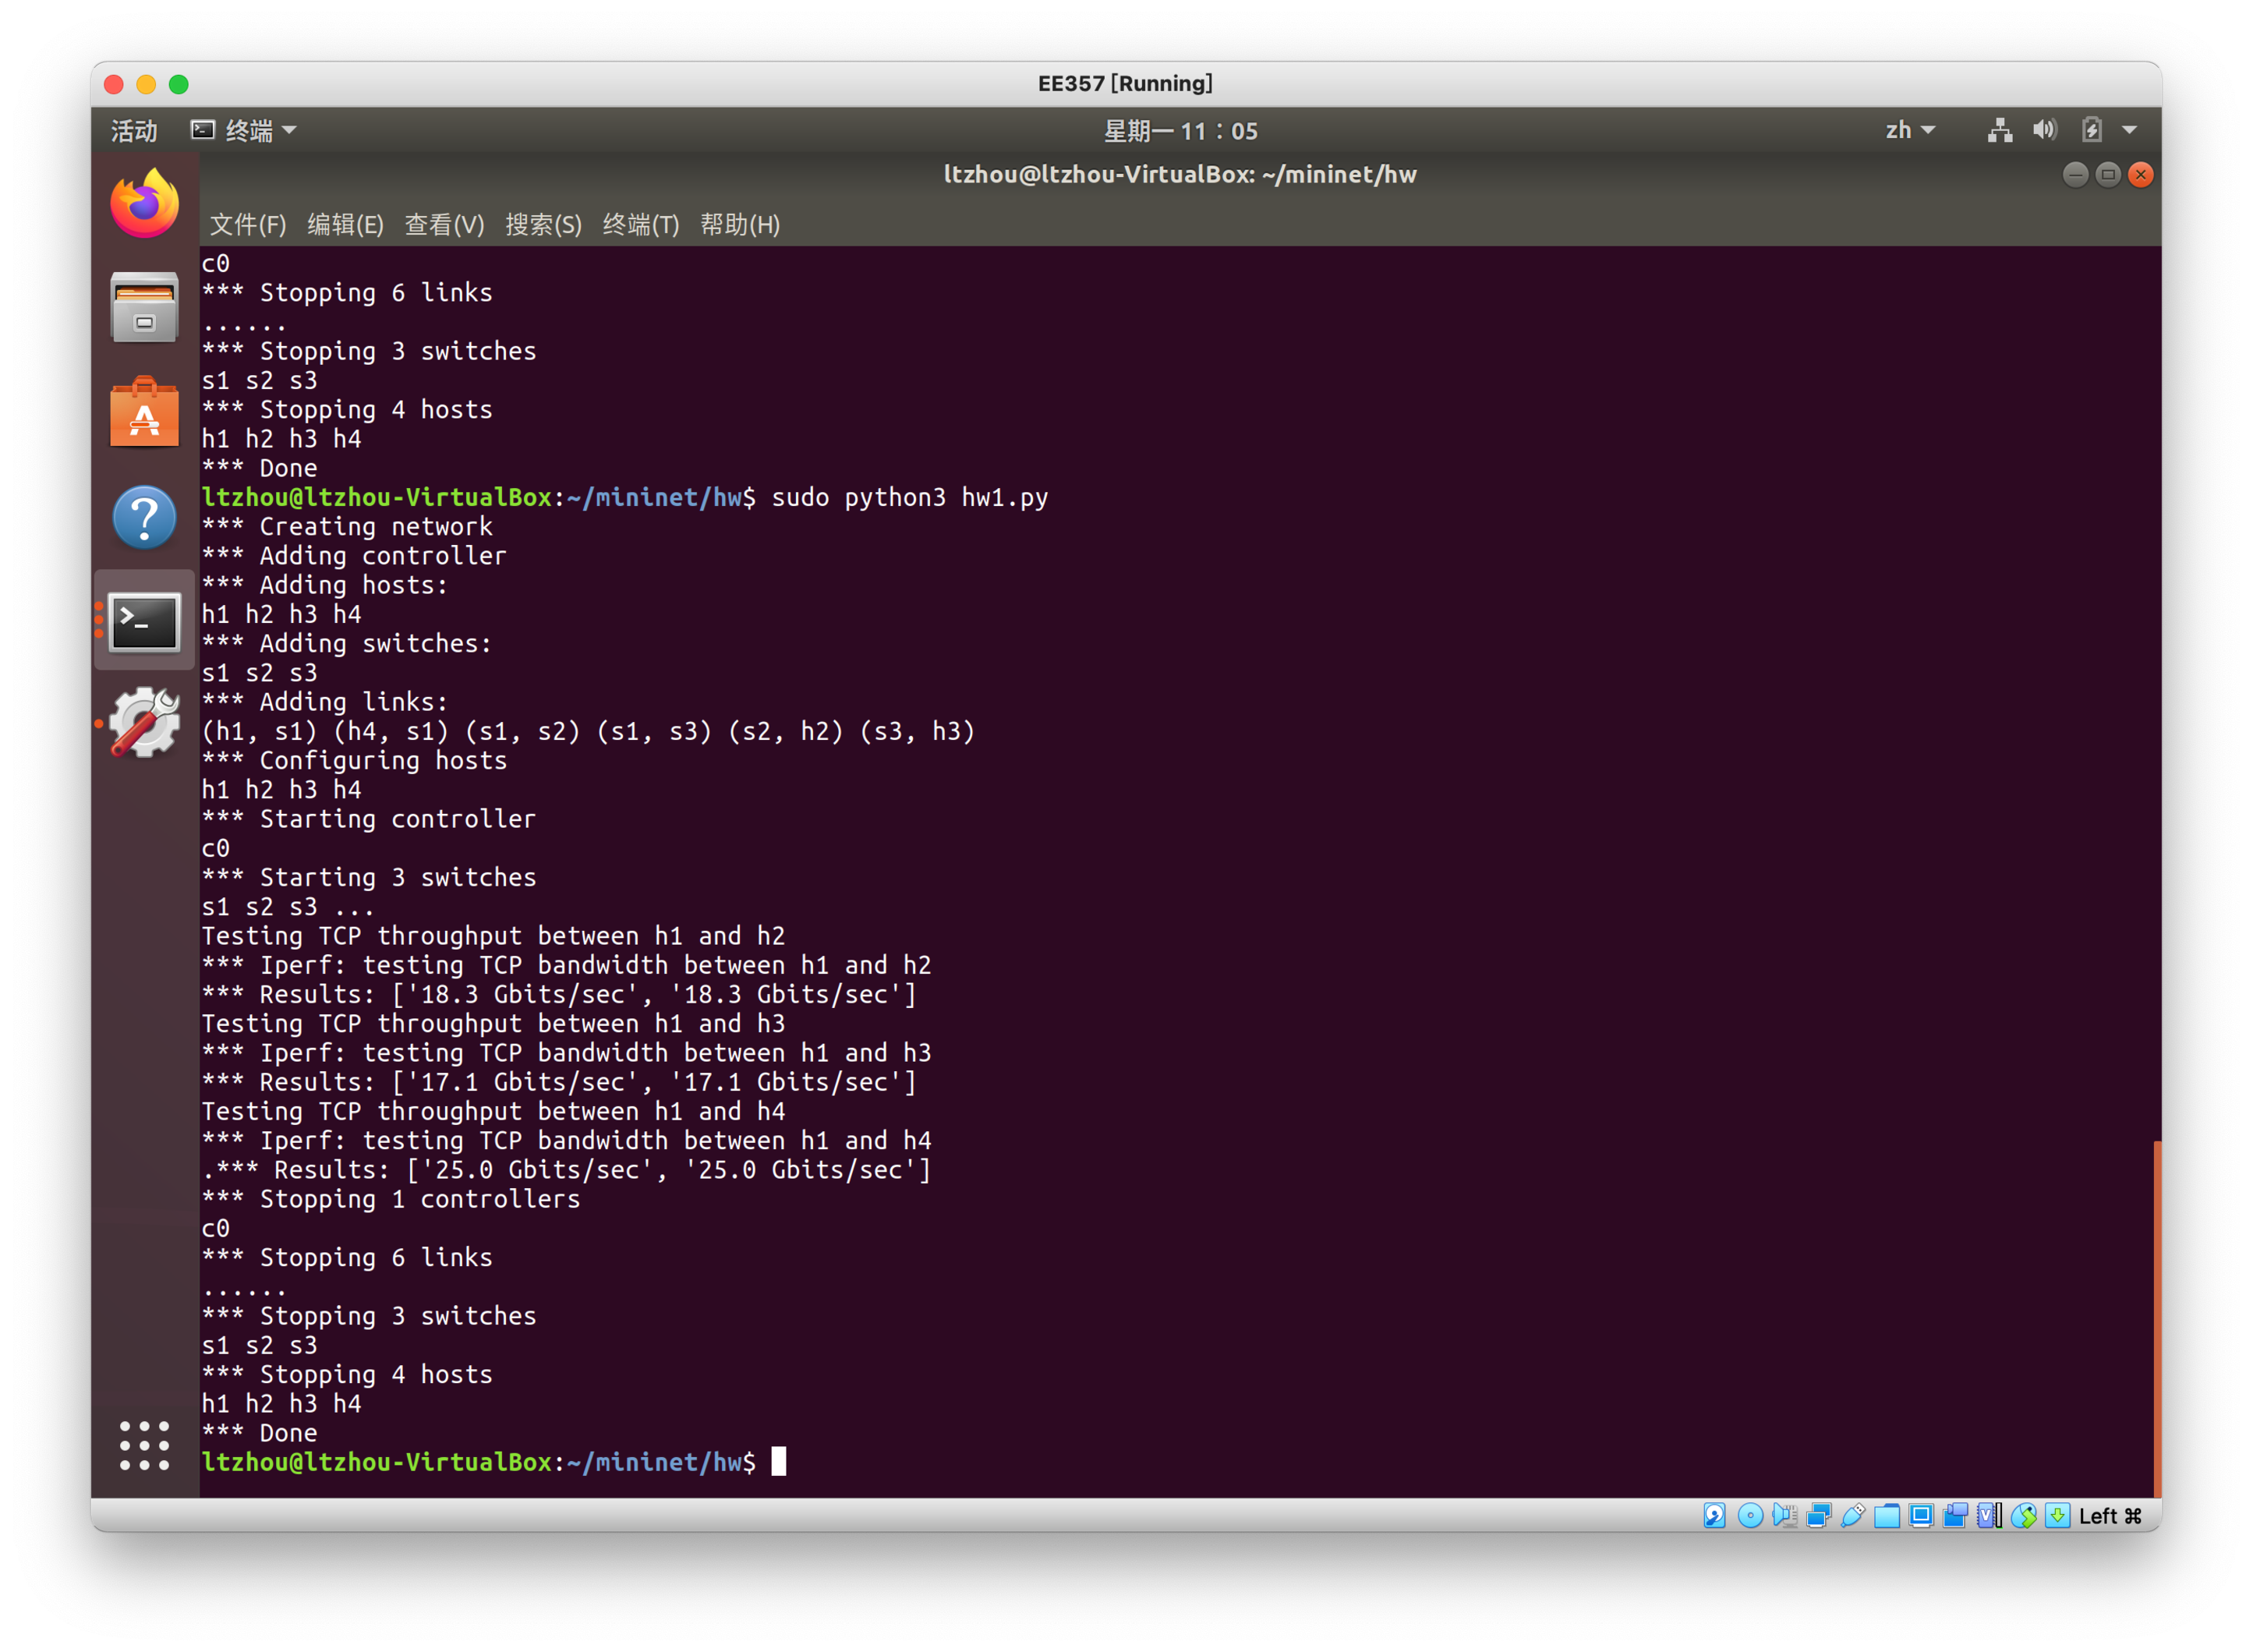
\includegraphics[width=12cm]{img/lab2/ex1}
  \caption{ipef3 test for the first exercise}
  \label{fig:ex1}
  \end{center}
\end{figure}

  \label{ex1}
\end{exercise}


%%%%%%%%%%%%%%%%%%%%%%%%%%%%%%%%%%%%%%%%%%
%%%%%%%%%%%%%                 %%%%%%%%%%%%
%%%%%%%%%%%%%    EXERCISE 2   %%%%%%%%%%%%
%%%%%%%%%%%%%                 %%%%%%%%%%%%
%%%%%%%%%%%%%%%%%%%%%%%%%%%%%%%%%%%%%%%%%%
\begin{exercise}[]{Now let us set the packet loss rate of the link (s1,s2) and (s1,s3) as 6\%. Use iperf3 to test the TCP throughput between h1 to h2, h3, h4 again.(30 points)}
  \begin{solution}
  \par{~}
  The TCP throughput between h1 to h2, h3, h4 is 24.3, 19.4 and 16.3 Gbits/sec respectively, shown in Figure \ref{fig:ex2}.
  
  \begin{figure}[hb]
    \begin{center}
    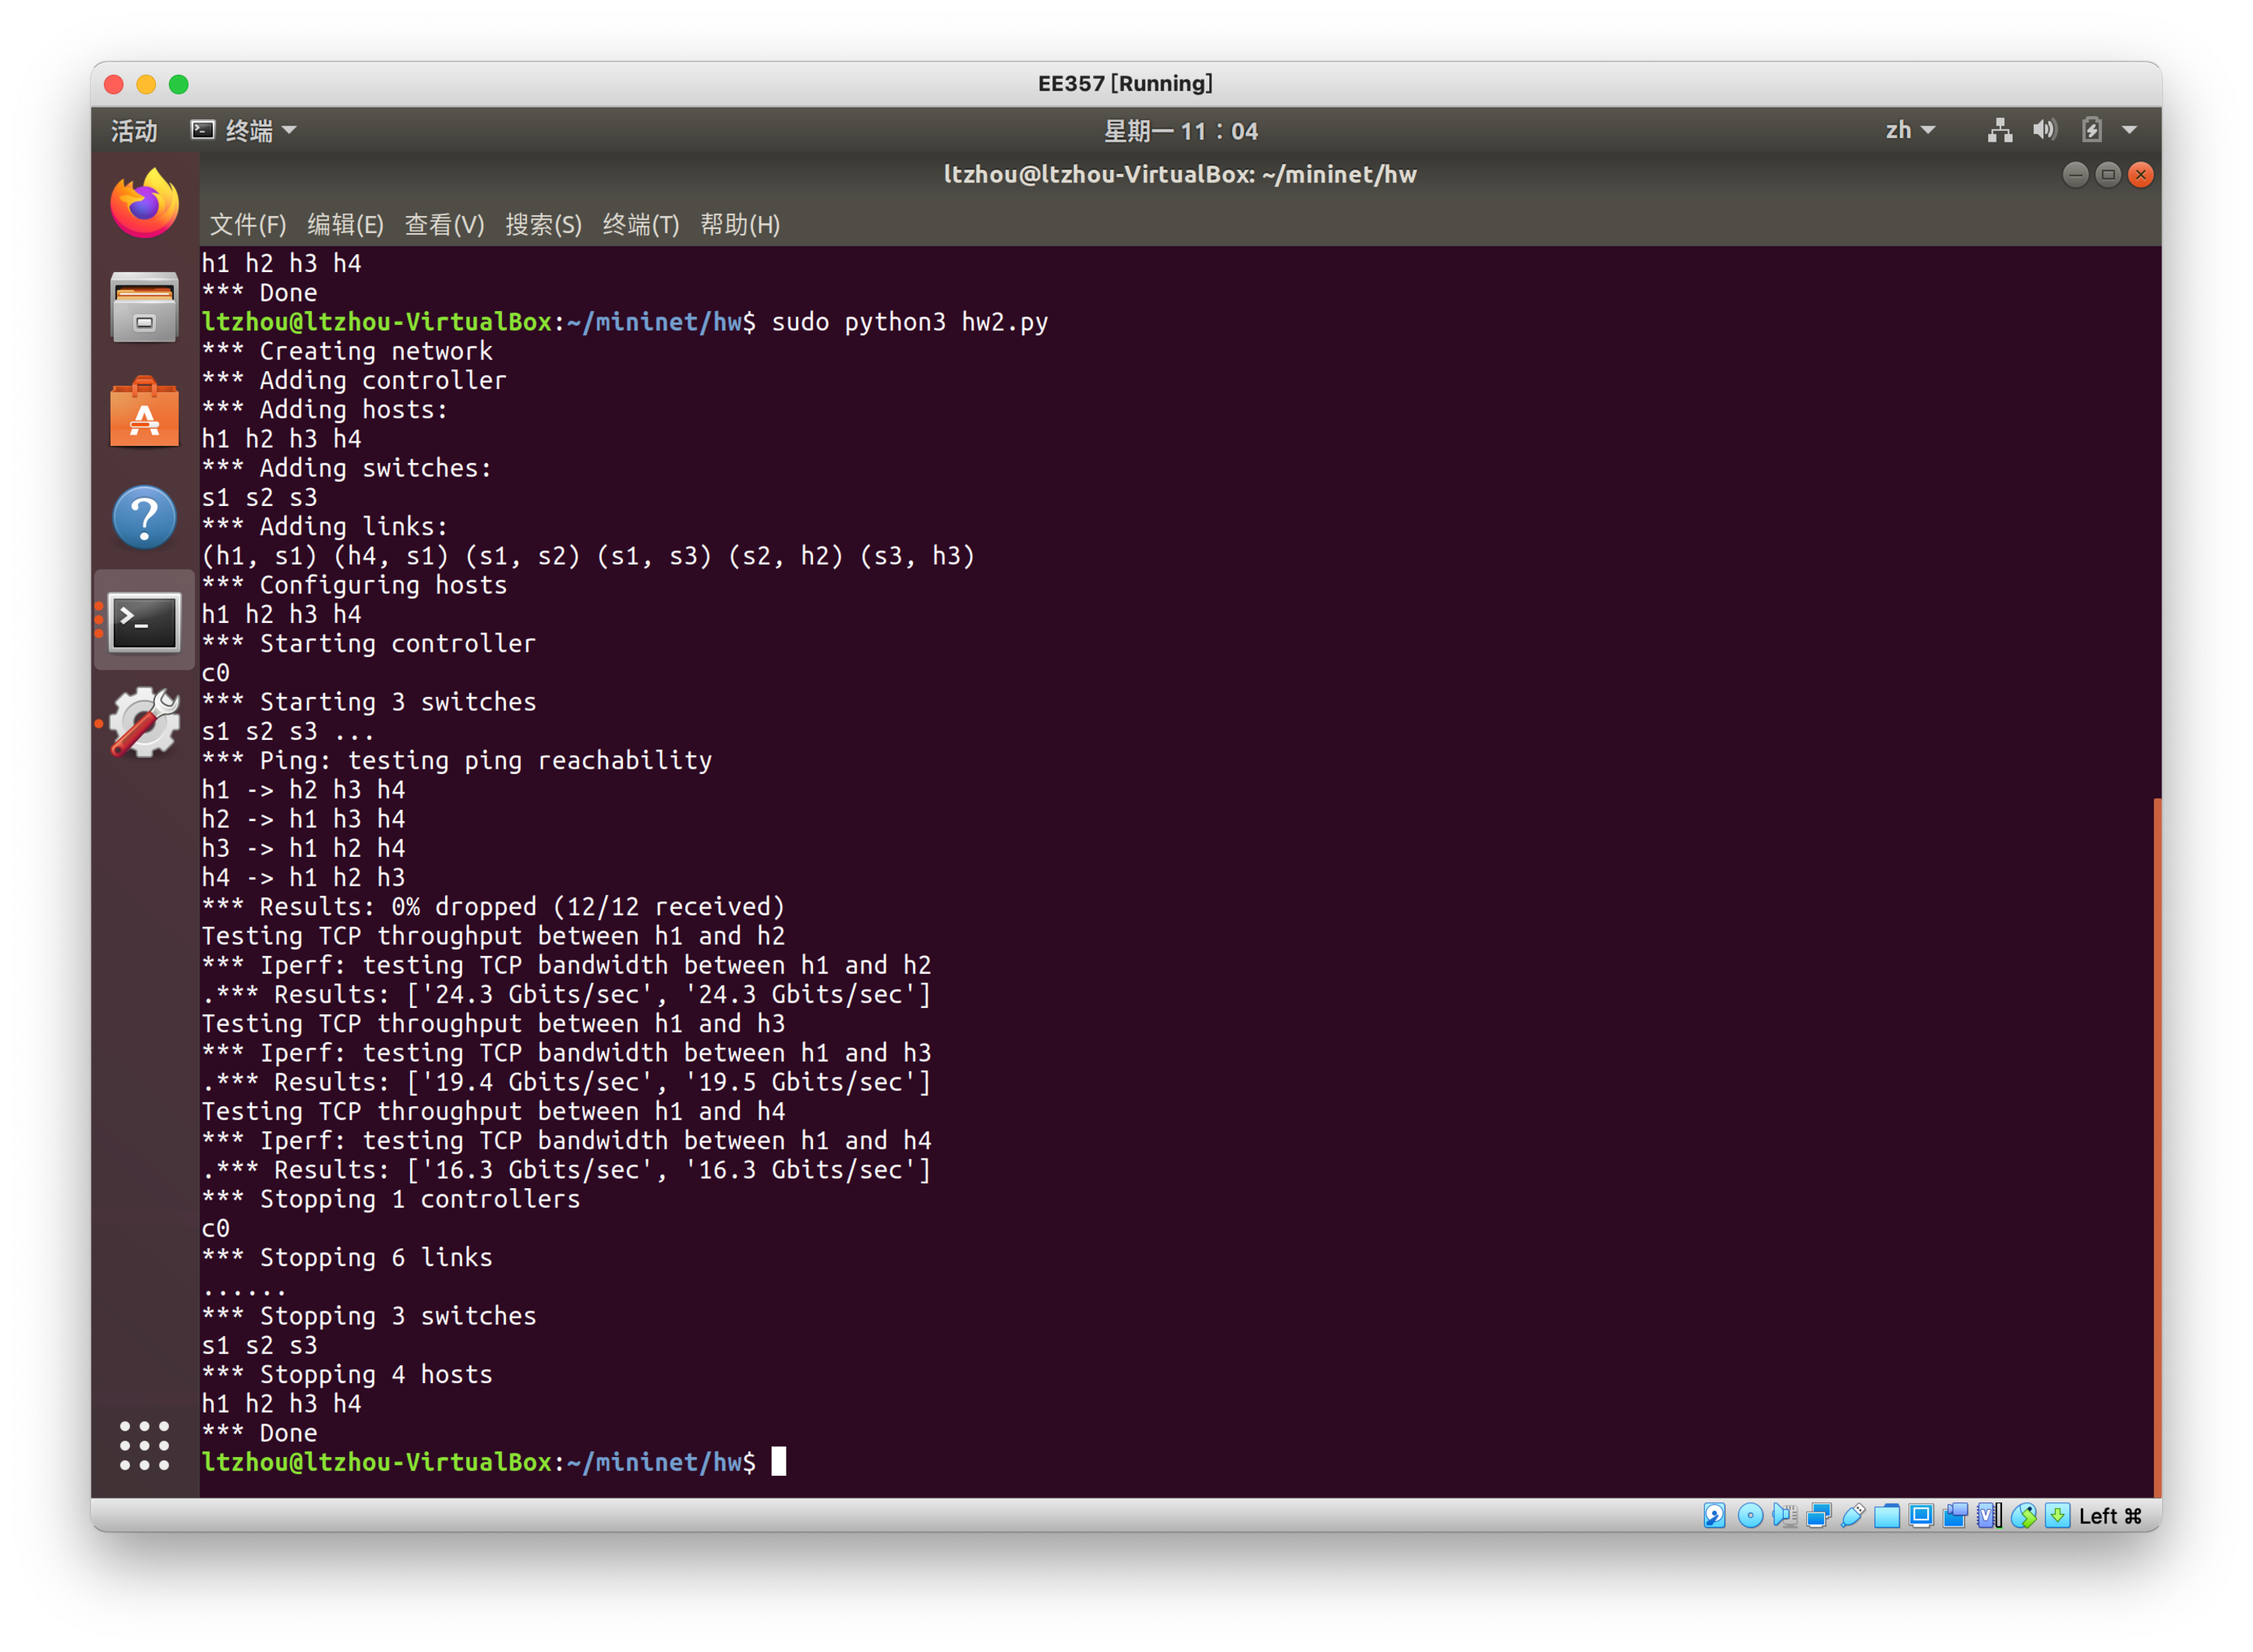
\includegraphics[width=12cm]{img/lab2/ex2}
    \caption{ipef3 test for the second exercise}
    \label{fig:ex2}
    \end{center}
  \end{figure}
  \end{solution}
  \label{ex2}
\end{exercise}


%%%%%%%%%%%%%%%%%%%%%%%%%%%%%%%%%%%%%%%%%%
%%%%%%%%%%%%%                 %%%%%%%%%%%%
%%%%%%%%%%%%%    EXERCISE 3   %%%%%%%%%%%%
%%%%%%%%%%%%%                 %%%%%%%%%%%%
%%%%%%%%%%%%%%%%%%%%%%%%%%%%%%%%%%%%%%%%%%
\begin{exercise}[]{Let us add another link between s2 and s3. Try to test the connectivity between all the hosts. What would happen? How would you solve the problem?(40 points)}
  \begin{solution}
  \par{~}

  The process of creating this topology can be found in Figure \ref{fig:ex3-1}. The pingall command shows that no data can be transferred from one host to another.

  This is because there exists a cycle of switches in the network, without any flooding control strategies. A \textbf{broadcasting storm} will happen. As broadcasts and multicasts are forwarded by switches out of every port, the switch or switches will repeatedly rebroadcast broadcast messages on the cycle and untimately flood the network, causing no data can be actually transferred to the other host any more.

  My solution in this problem is to disable one of the edge to eliminate the loop by using \texttt{ovs-ofctl} command. I proposed two solutions in solving this problem. Both solutions managed to eliminate the use of a link in the cycle either by dropping all packets received from the link or by not sending any packets to that link. See Figure \ref{code:sol1} and Figure \ref{code:sol2}. Now the \texttt{pingall} can work again. See Figure \ref{fig:ex3-2}





  \end{solution}
  \label{ex3}
\end{exercise}



\begin{figure}[!h]
    \caption{Solution 1: disable all output to a link in the loop}
    \label{code:sol1}
\begin{lstlisting}[language=C,frame=single]
sudo ovs-ofctl add-flow s1 "in_port=s1-eth4 actions=drop"                    # s2 --x-> s1
sudo ovs-ofctl add-flow s2 "in_port=s2-eth1 actions=drop"                    # s1 --x-> s2
\end{lstlisting}
\end{figure}



\begin{figure}[!h]
    \caption{Solution 2: disable all input to a link in the loop}
    \label{code:sol2}
\begin{lstlisting}[language=C,frame=single]
sudo ovs-ofctl add-flow s2 "in_port=s2-eth1 actions=s2-eth2"                    # s1 -> s2 -> h2
sudo ovs-ofctl add-flow s3 "in_port=s3-eth1 actions=s3-eth2"                    # s1 -> s3 -> h3
sudo ovs-ofctl add-flow s2 "in_port=s2-eth2 actions=s2-eth1"                    # h2 -> s2 -> s1
sudo ovs-ofctl add-flow s3 "in_port=s3-eth2 actions=s3-eth1"                    # h3 -> s3 -> s1
\end{lstlisting}
\end{figure}


\begin{figure}[hb]
  \begin{center}
  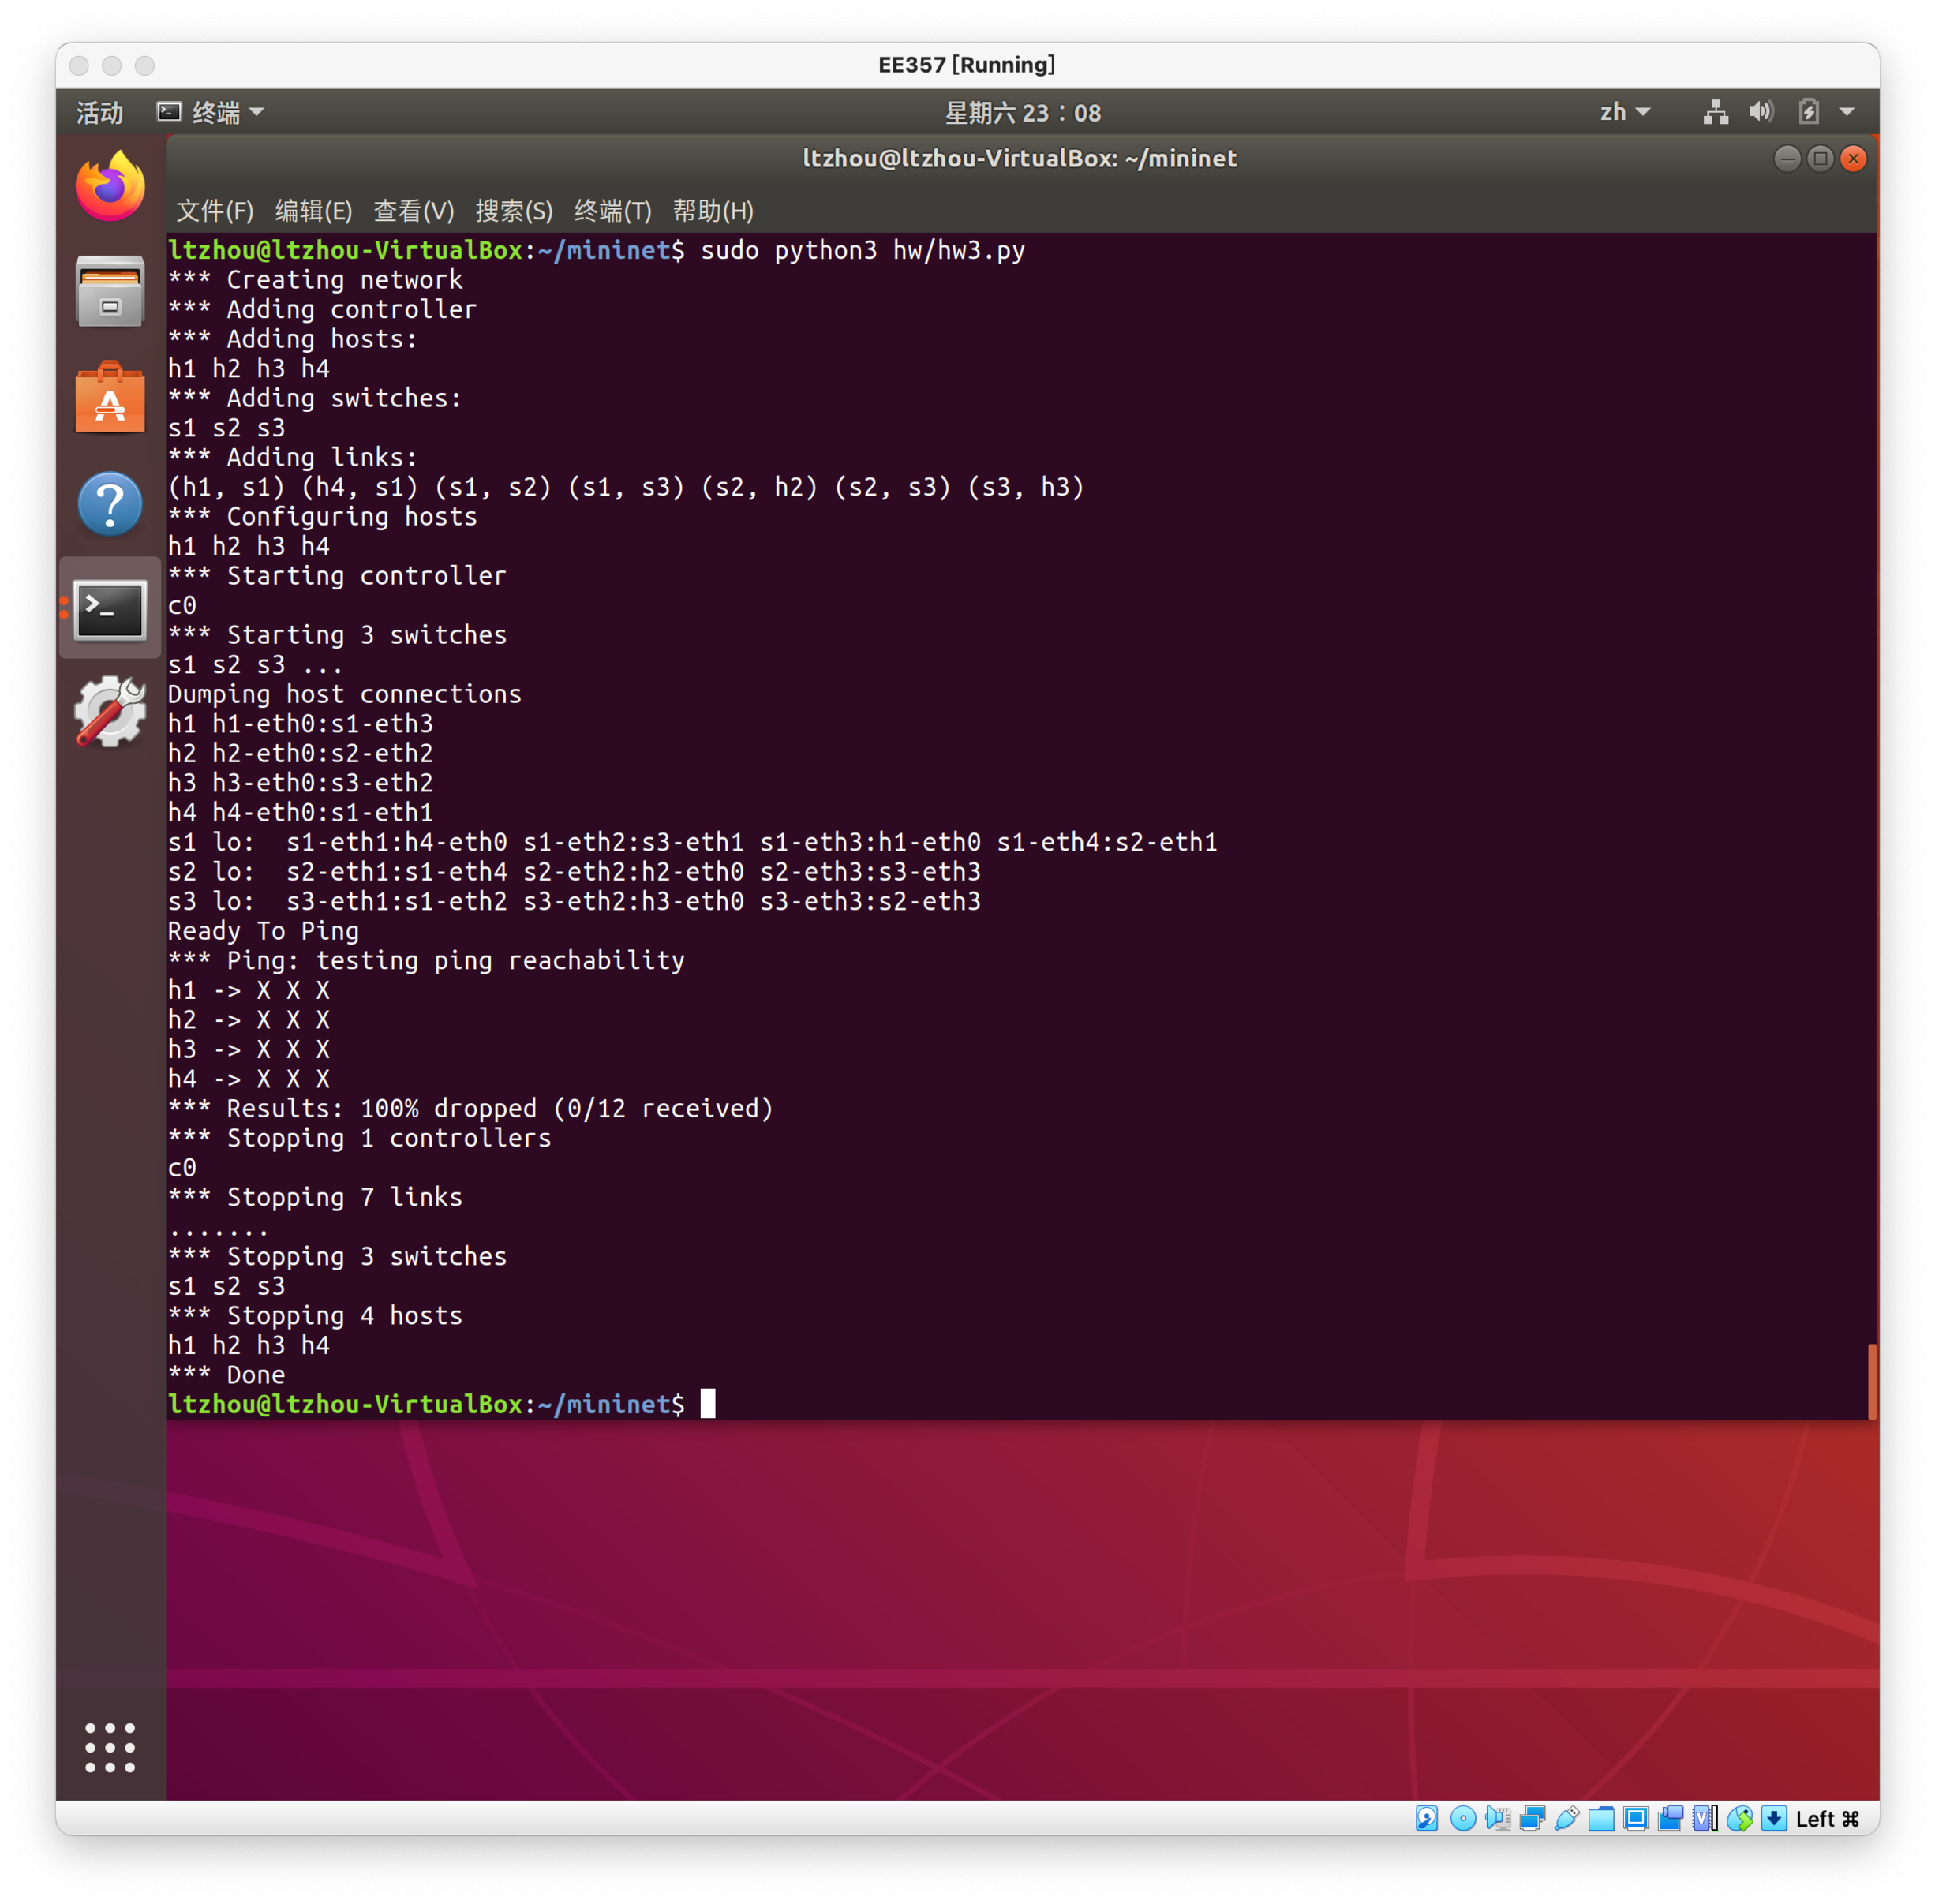
\includegraphics[width=12cm]{img/lab2/ex3-1}
  \caption{pingall fails on loop switches}
  \label{fig:ex3-1}
  \end{center}
\end{figure}

\begin{figure}[hb]
    \begin{center}
    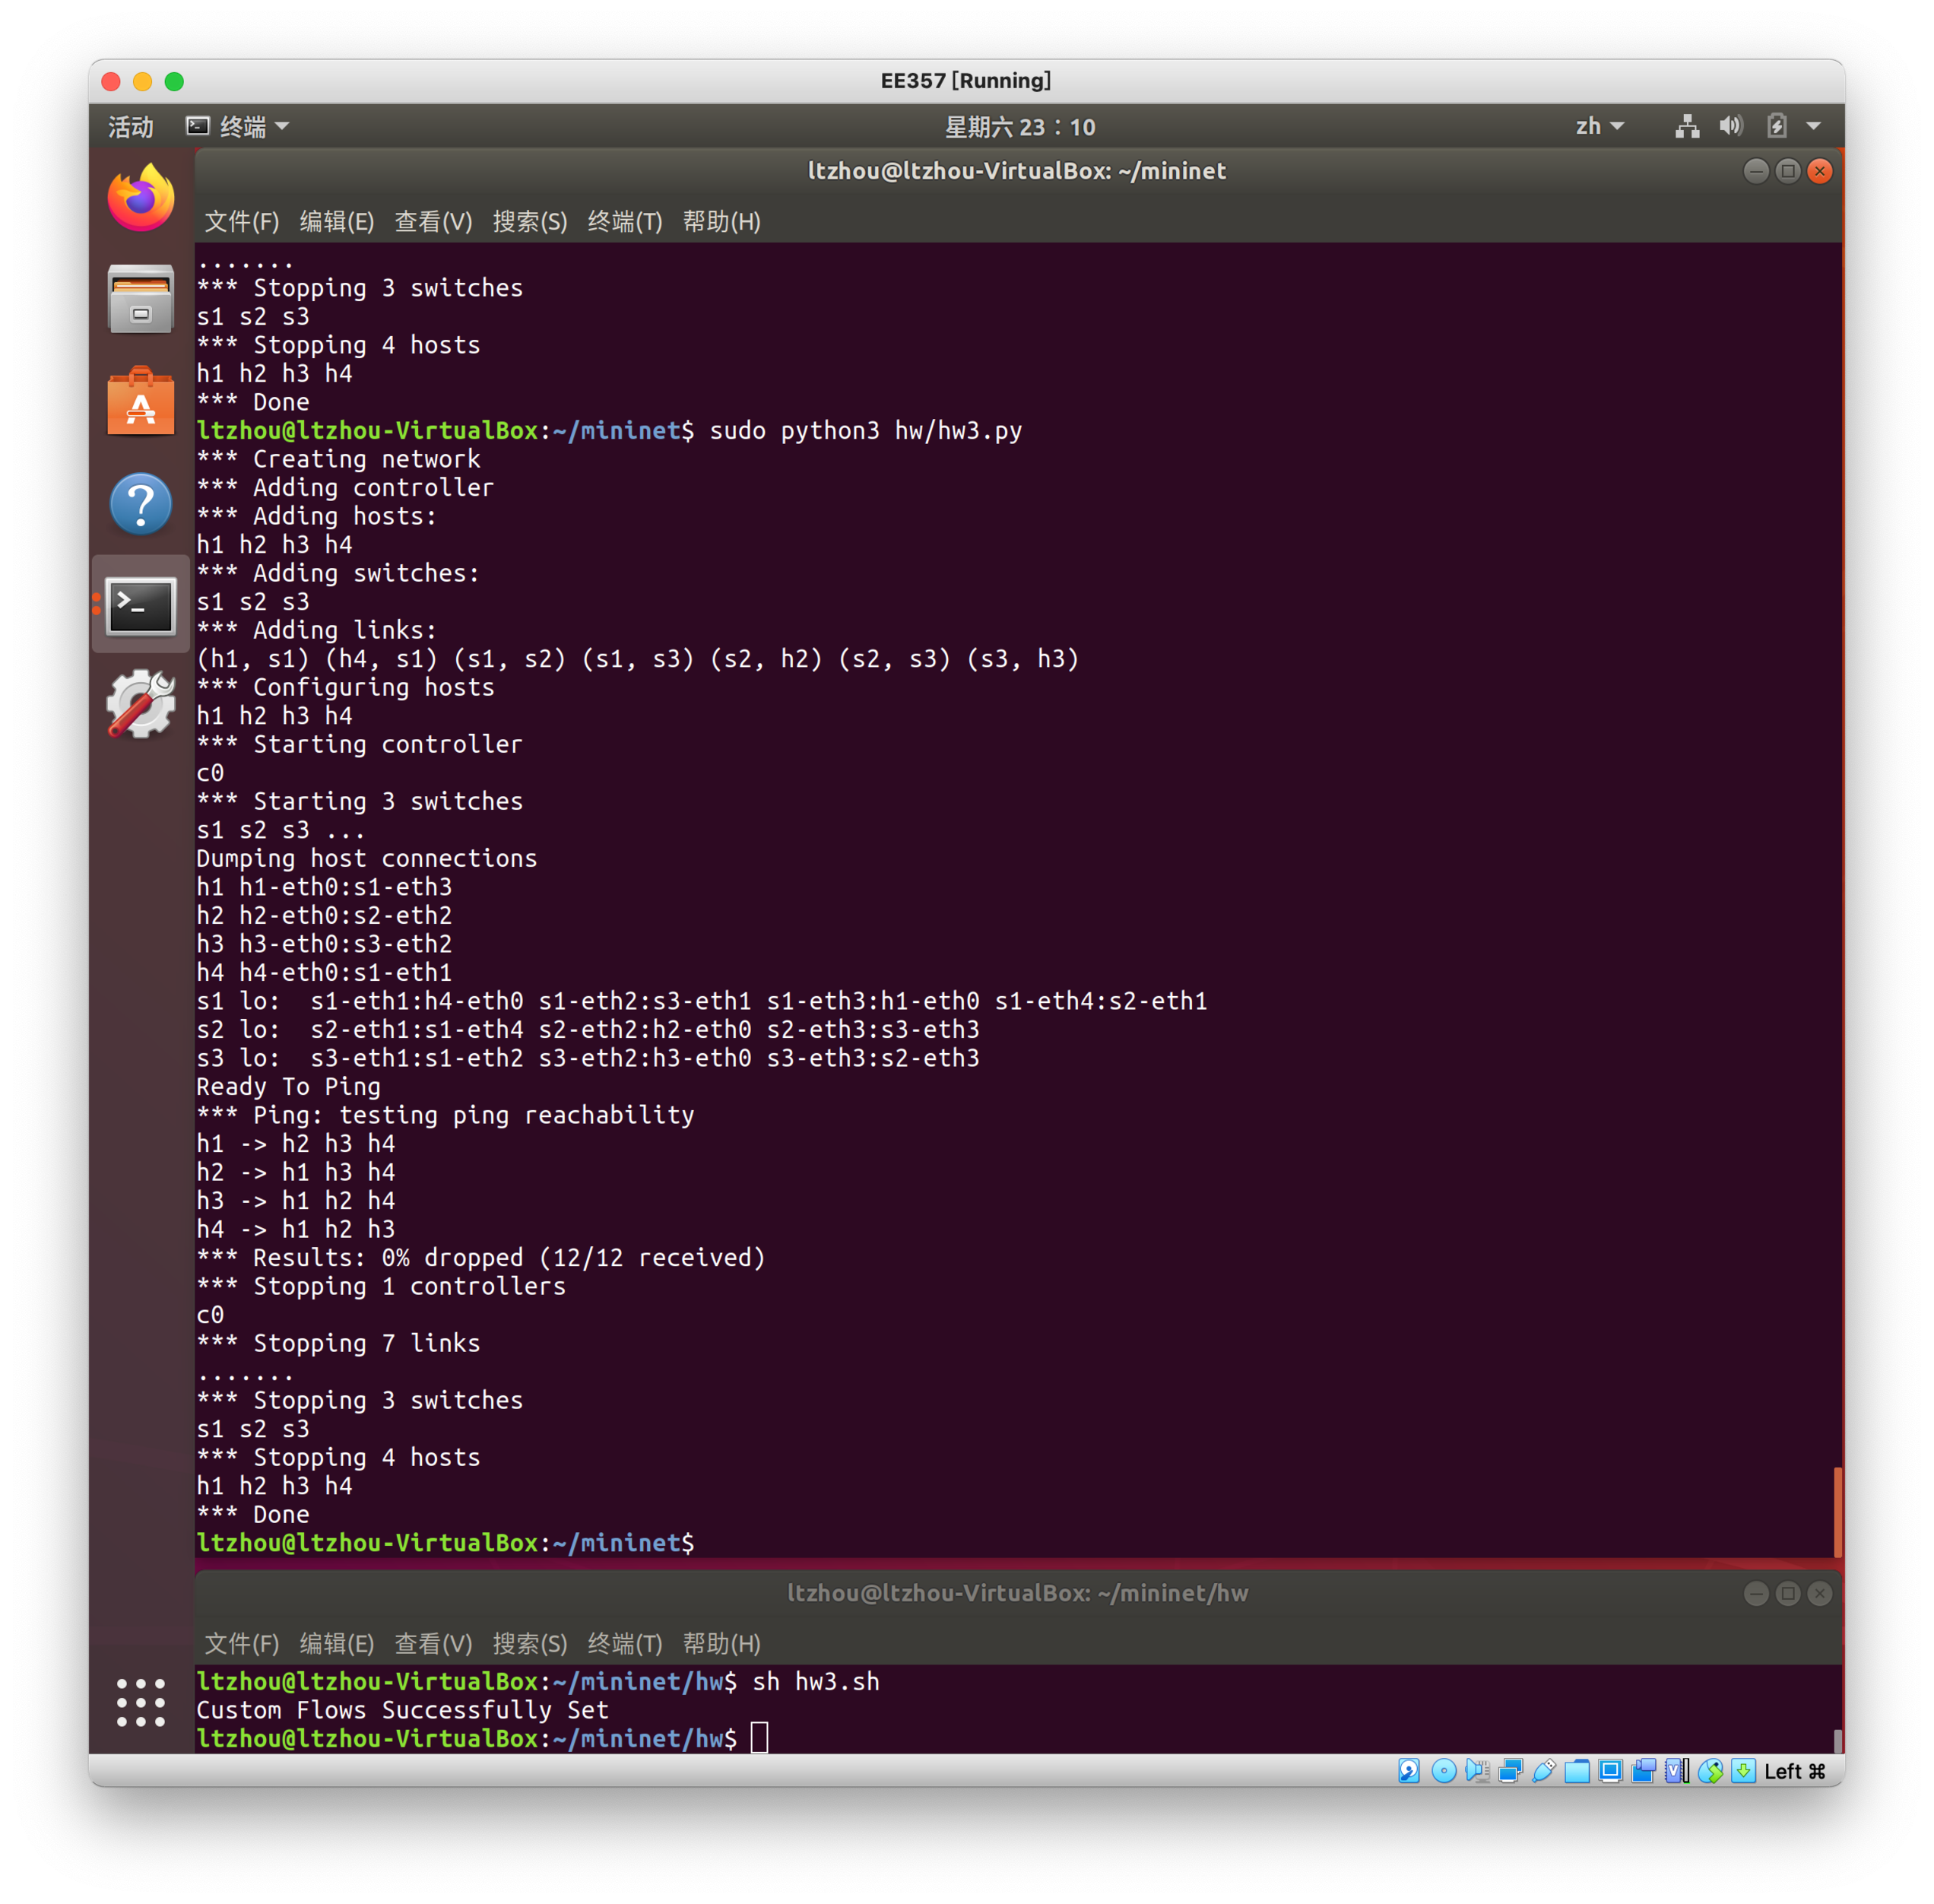
\includegraphics[width=12cm]{img/lab2/ex3-2}
    \caption{pingall works again after flow-control}
    \label{fig:ex3-2}
    \end{center}
  \end{figure}